\documentclass[10pt]{article}
\usepackage{mathpazo}
\usepackage{tabularx,amsmath,boxedminipage}
\usepackage{graphicx}				% enables graphics
\graphicspath{ {images/} }			% sets graphics path
\usepackage[margin=1in,letterpaper]{geometry} % this shaves off default margins which are too big
\usepackage{cite}
\usepackage{sectsty}
\usepackage{setspace}
\setlength\parindent{0pt}			% sets no indents
\usepackage{float}
\makeatletter						% set figure labels to center
\g@addto@macro\@floatboxreset\centering
\makeatother
\usepackage[labelsep=endash, labelfont=bf]{caption}	% sets figure and caption separator
\usepackage[framed]{mcode}
\usepackage{enumitem}
\usepackage[final]{hyperref} % adds hyper links inside the generated pdf file
\hypersetup{
	colorlinks=false,       % false: boxed links; true: colored links
	linkcolor=blue,          % color of internal links
	citecolor=blue,        % color of links to bibliography
	filecolor=magenta,      % color of file links
	urlcolor=blue         
}
\usepackage{titlesec}				% enables title formatting
\titleformat{\part}{\filright\huge\bfseries}{}{}{}
\setlength{\parskip}{0.5em}			% sets paragraph spacing to 1m
\newcommand{\pder}[2]{\dfrac{\partial#1}{\partial#2}}			% partial command

\begin{document}

\newcommand{\stoptocwriting}{%
	\addtocontents{toc}{\protect\setcounter{tocdepth}{-5}}}
\newcommand{\resumetocwriting}{%
	\addtocontents{toc}{\protect\setcounter{tocdepth}{\arabic{tocdepth}}}}

\stoptocwriting
\part*{\underline{AERO 430 -- Numerical Solution} \\ \Large Homework 1 -- Solution}

\vspace{80 pt}

\begin{center}
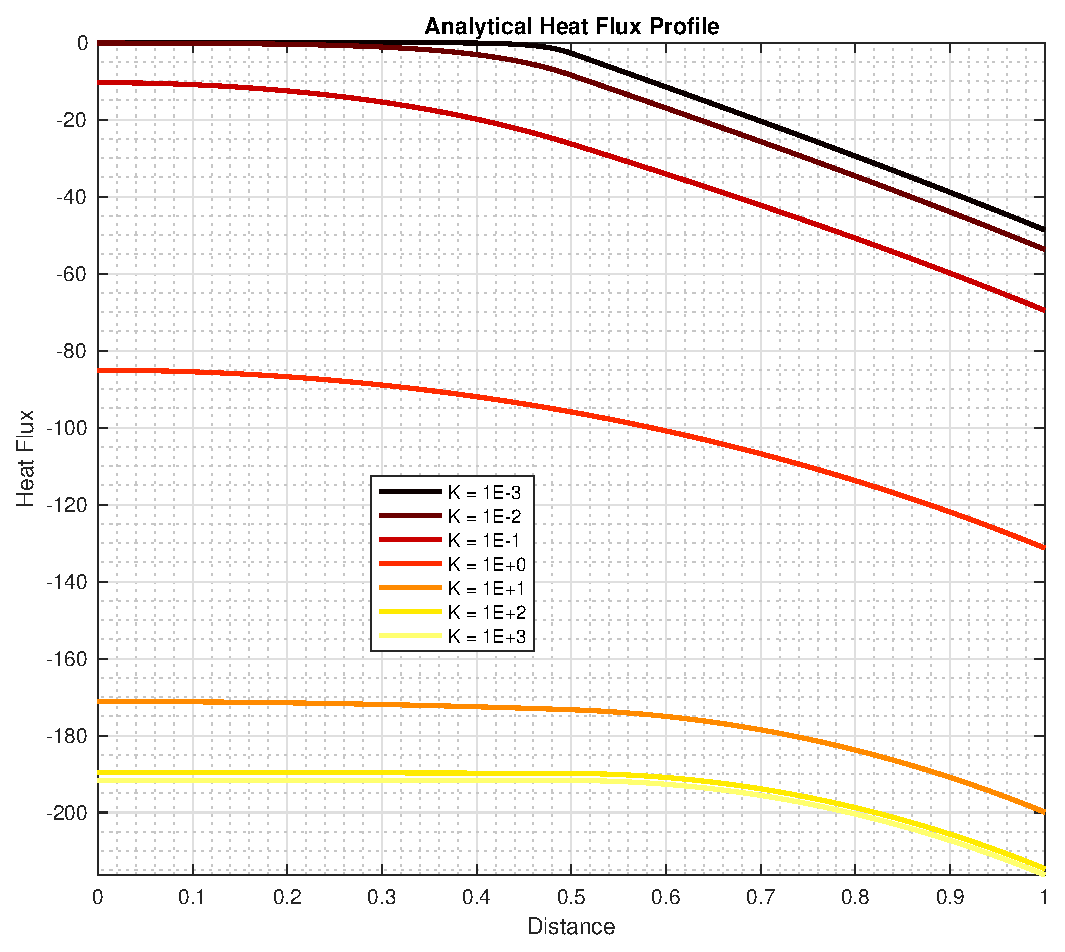
\includegraphics[width=0.7\linewidth]{aero_430_hw1_analytical_heat_flux}
\end{center}

\vfill

\begin{flushleft}
	\large Ross Alexander \\ 2.11.18
\end{flushleft}
\resumetocwriting

\newpage

\section*{Analytical Solution}

For the given problem, the governing equation is:
\begin{equation}
-u'' + \frac{b}{k}u = 0 \qquad x \in [0, 1]
\end{equation}
Since the differential equation is split into two regions with different coefficients, the governing equations become:
\begin{equation}
-u'' + \alpha_1^2u = 0 \qquad x \in [0, \tfrac{1}{2}]
\end{equation}
\begin{equation}
-u'' + \alpha_2^2u = 0 \qquad x \in [\tfrac{1}{2}, 1]
\end{equation}
with $\alpha_i^2 = \frac{b}{k_i}$.
The boundary conditions are temperatures at the left and right ends of the domain, 0 and 100, respectively, and the continuity conditions for temperature and heat flux ($\dot{Q}=-kAu'$) at the midpoint of the domain:
\begin{equation}
\begin{split}
u(0) = 0  \qquad \qquad \qquad \qquad \qquad  \; u(1) = 100 \\
u(\tfrac{1}{2}) = u(\tfrac{1}{2}) \qquad -k_1Au'(\tfrac{1}{2}) = -k_2Au'(\tfrac{1}{2})
\end{split}
\end{equation}

The general solution for the second-order inhomogeneous partial differential equation of similar form is:
\begin{equation}
u(x) = A\cosh(\alpha x) + B\sinh(\alpha x) + C
\end{equation}
In the case of this problem, we have:
\begin{equation}
u_1(x) = A\cosh(\alpha_1 x) + B\sinh(\alpha_1 x) + T_a \qquad x \in [0, \tfrac{1}{2}]
\end{equation}
\begin{equation}
u_2(x) = C\cosh(\alpha_2 x) + D\sinh(\alpha_2 x) + T_a \qquad x \in [\tfrac{1}{2}, 1]
\end{equation}
A straightforward application of the boundary conditions and the use of a numerical solver yields the coefficients A, B, C, and D. For conditions $b=1$, $k_1=K*k_2$, $k_2=1$, $T_a=0$, $A=1$, and for $K \in \{10^{-3}, 10^{-2}, 10^{-1}, 10^{+0}, 10^{+1}, 10^{+2}, 10^{+3}\}$, the analytical temperature and heat flux profiles are calculated below.

\vfill

\begin{figure}[H]
	\begin{center}
		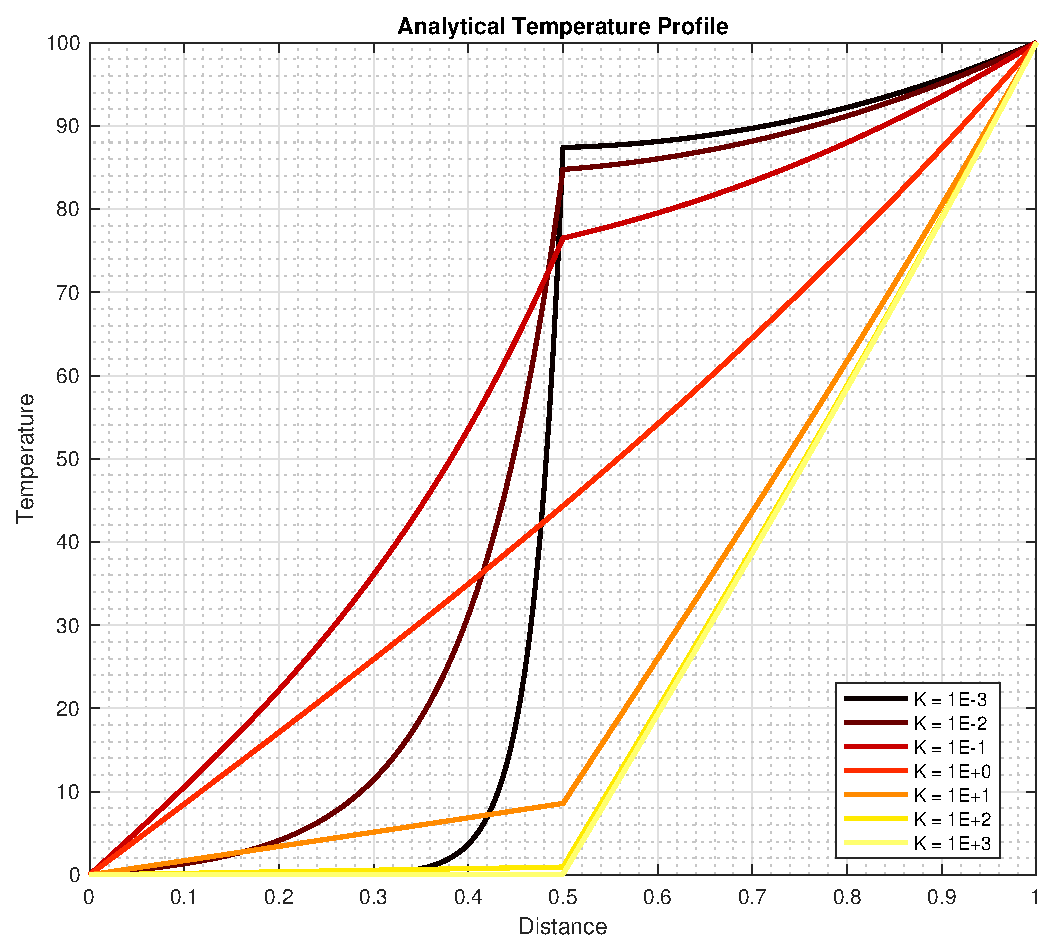
\includegraphics[width=0.497\linewidth]{aero_430_hw1_analytical_temperature}
		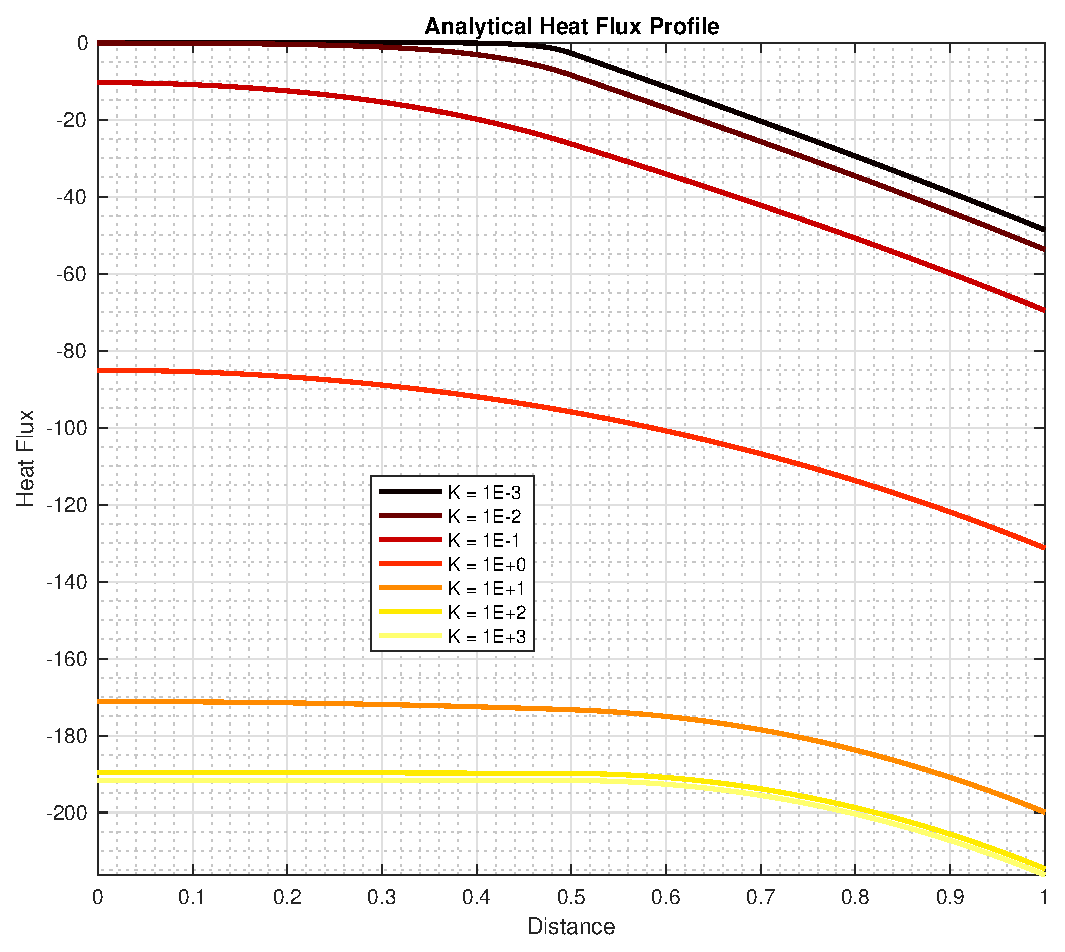
\includegraphics[width=0.497\linewidth]{aero_430_hw1_analytical_heat_flux}
		\caption{Analytical Temperature and Heat Flux Profiles}
	\end{center}
\end{figure}

\newpage

\section*{Finite Difference Method}

\subsection*{2nd-Order Central Difference Scheme}
The second-order discretization scheme is achieved using the heat flux gradient form of the governing equation, where $Q = -ku'$ and $Q' = -ku''$:
\begin{equation}
Q' + bu = 0
\end{equation}
Or in discrete form:
\begin{equation}
Q'_i + b_iu_i = 0
\end{equation}
First the heat flux gradient is discretized using the midpoints, rearranged, and then exchanged for the temperature gradients:
\begin{equation}
\frac{Q_{i+\tfrac{1}{2}}-Q_{i-\tfrac{1}{2}}}{\Delta x} + b_iu_i=0
\end{equation}
\begin{equation}
Q_{i+\tfrac{1}{2}}-Q_{i-\tfrac{1}{2}} + b_iu_i\Delta x=0
\end{equation}
\begin{equation}
-k_{i+\tfrac{1}{2}}u'_{i+\tfrac{1}{2}}+k_{i-\tfrac{1}{2}}u'_{i-\tfrac{1}{2}} + b_iu_i\Delta x=0
\end{equation}
Then, the temperature gradients are discretized using the nodes and rearranged:
\begin{equation}
-k_{i+\tfrac{1}{2}}\frac{u_{i+1}-u_i}{\Delta x} + k_{i-\tfrac{1}{2}}\frac{u_i-u_{i-1}}{\Delta x} + b_iu_i\Delta x=0
\end{equation}
\begin{equation}
-k_{i+\tfrac{1}{2}}(u_{i+1}-u_i) + k_{i-\tfrac{1}{2}}(u_i-u_{i-1}) + b_iu_i\Delta x^2=0
\end{equation}
Simplifying yields the three-point second-order stencil:
\begin{equation}
\mathbf{\left(-k_{i-\tfrac{1}{2}}\right)u_{i-1} + \left(b_i\Delta x^2 +k_{i-\tfrac{1}{2}} +k_{i+\tfrac{1}{2}} \right)u_{i} + \left(-k_{i+\tfrac{1}{2}}\right)u_{i+1}}
\end{equation}

\subsection*{2nd-Order Extraction Scheme}
Since the quanties of interest are $u(\tfrac{1}{2})$ and $Q(\tfrac{1}{2})$, formulas must be developed to extract them from the numerical results. However, this is trivial for $u(\tfrac{1}{2})$ since it is obtained directly from the numerical results. But, for the midpoint heat flux $Q(\tfrac{1}{2})$, a second-order extraction formula must be developed.

The two choices are to evaluate the heat flux using a forward or backward difference. Both formulas are given below:
\begin{equation}
\mathbf{Q(\tfrac{1}{2})^- = -k_{i-\tfrac{1}{2}}\frac{u_i-u_{i-1}}{\Delta x}-\frac{b\Delta x}{2}u_i}
\end{equation}
\begin{equation}
\mathbf{Q(\tfrac{1}{2})^+ = -k_{i+\tfrac{1}{2}}\frac{u_{i+1}-u_{i}}{\Delta x}+\frac{b\Delta x}{2}u_i}
\end{equation}

\newpage

\section*{Results}

\subsection*{Finite Difference Method}

A legend is provided for the figures below:
\begin{figure}[H]
	\begin{center}
		\includegraphics[width=0.15\linewidth]{legend}
	\end{center}
\end{figure}
\vfill
\begin{figure}[H]
	\begin{center}
		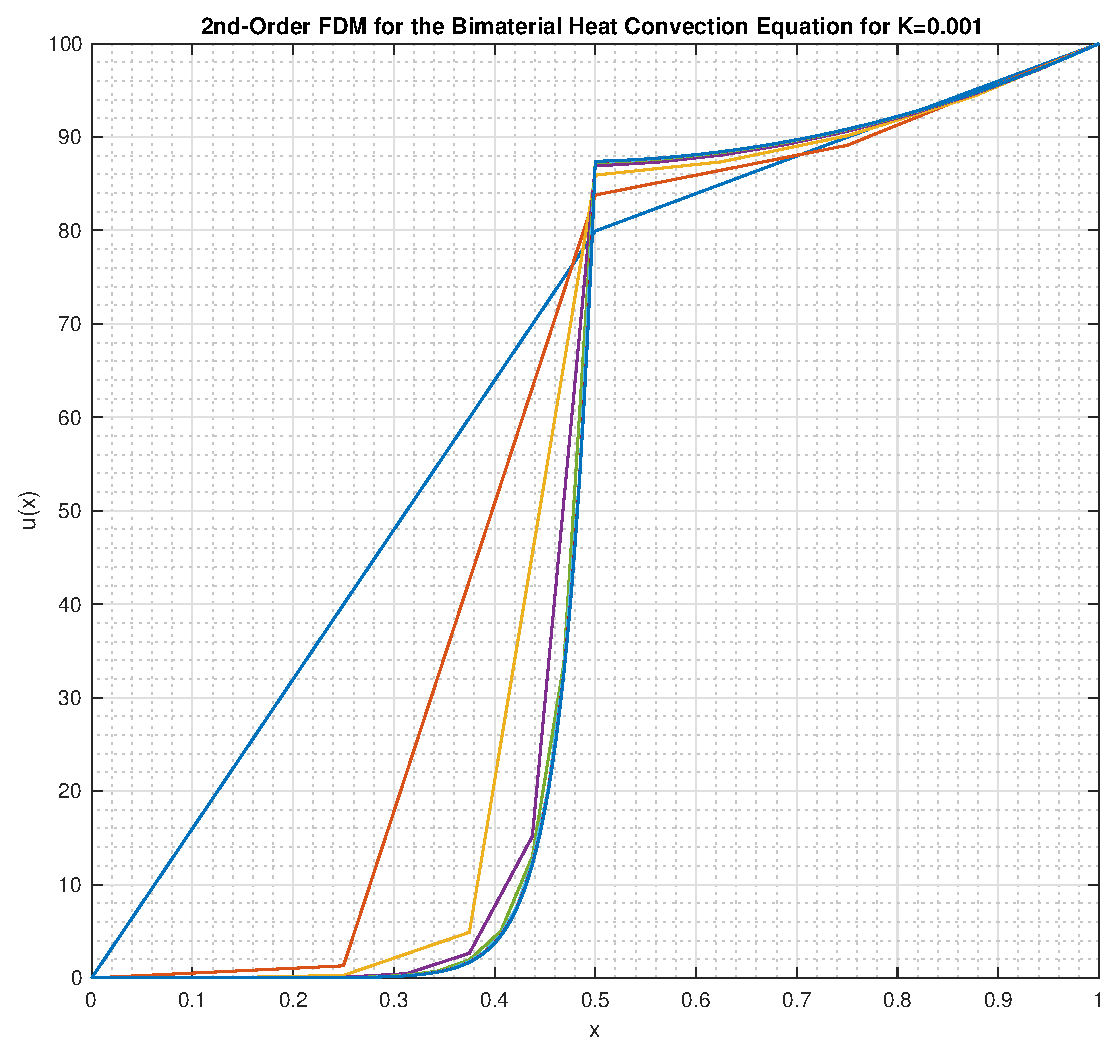
\includegraphics[width=0.6\linewidth]{solution_K_0001}
		\caption{FDM Solution for the Bimaterial Heat Convection Equation for K = 1E-3}
	\end{center}
\end{figure}

\begin{figure}[H]
	\begin{center}
		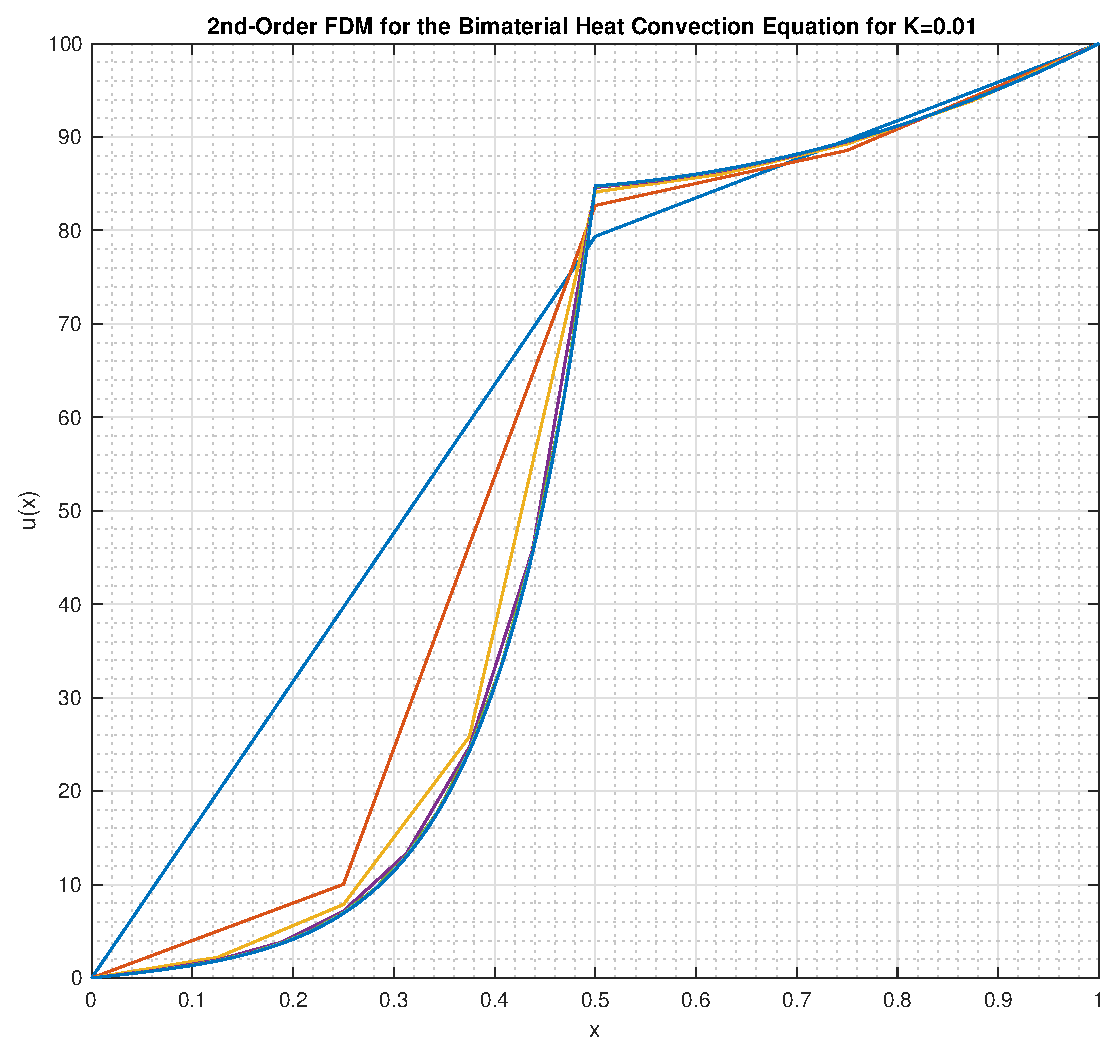
\includegraphics[width=0.6\linewidth]{solution_K_001}
		\caption{FDM Solution for the Bimaterial Heat Convection Equation for K = 1E-2}
	\end{center}
\end{figure}
\vfill
\begin{figure}[H]
	\begin{center}
		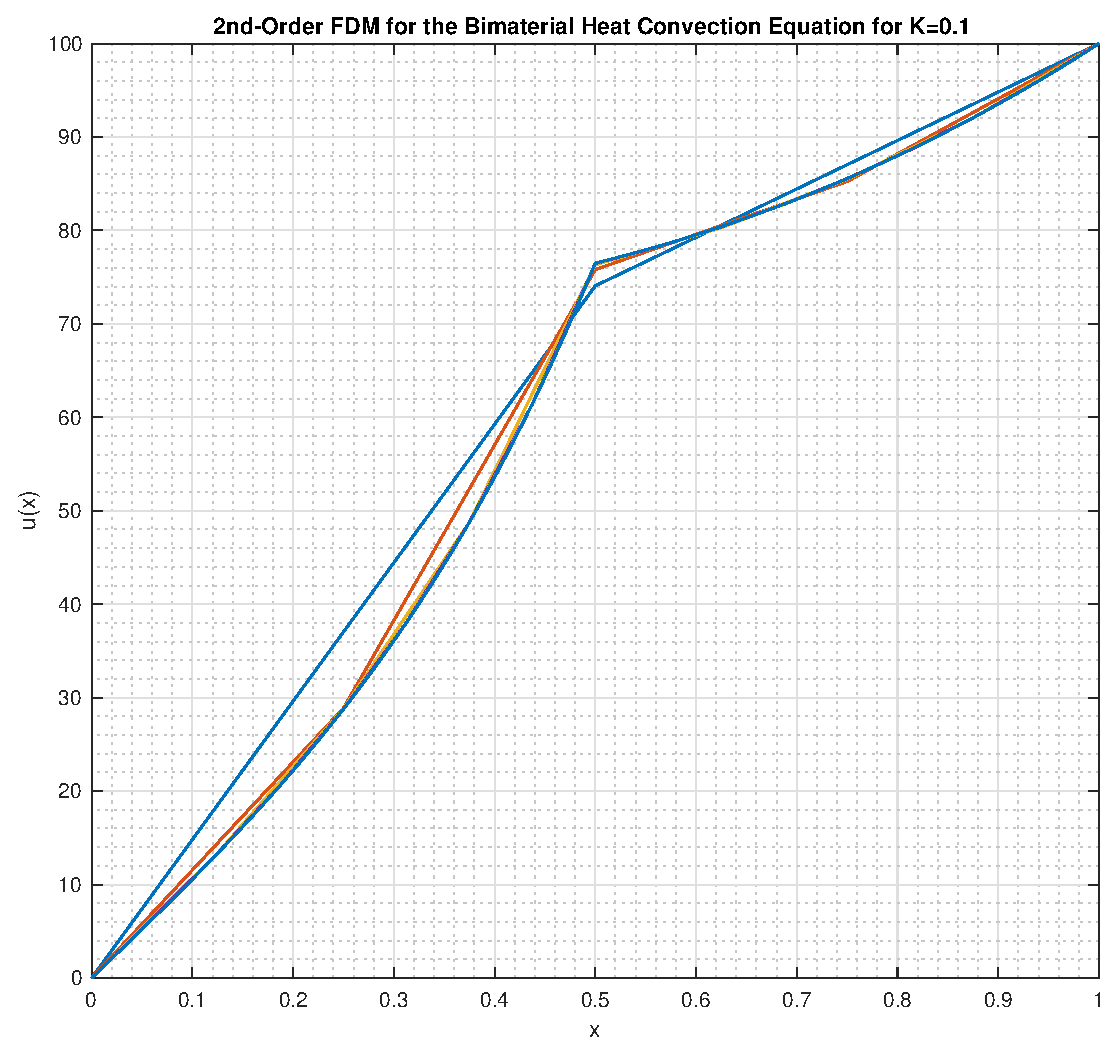
\includegraphics[width=0.6\linewidth]{solution_K_01}
		\caption{FDM Solution for the Bimaterial Heat Convection Equation for K = 1E-1}
	\end{center}
\end{figure}

\begin{figure}[H]
	\begin{center}
		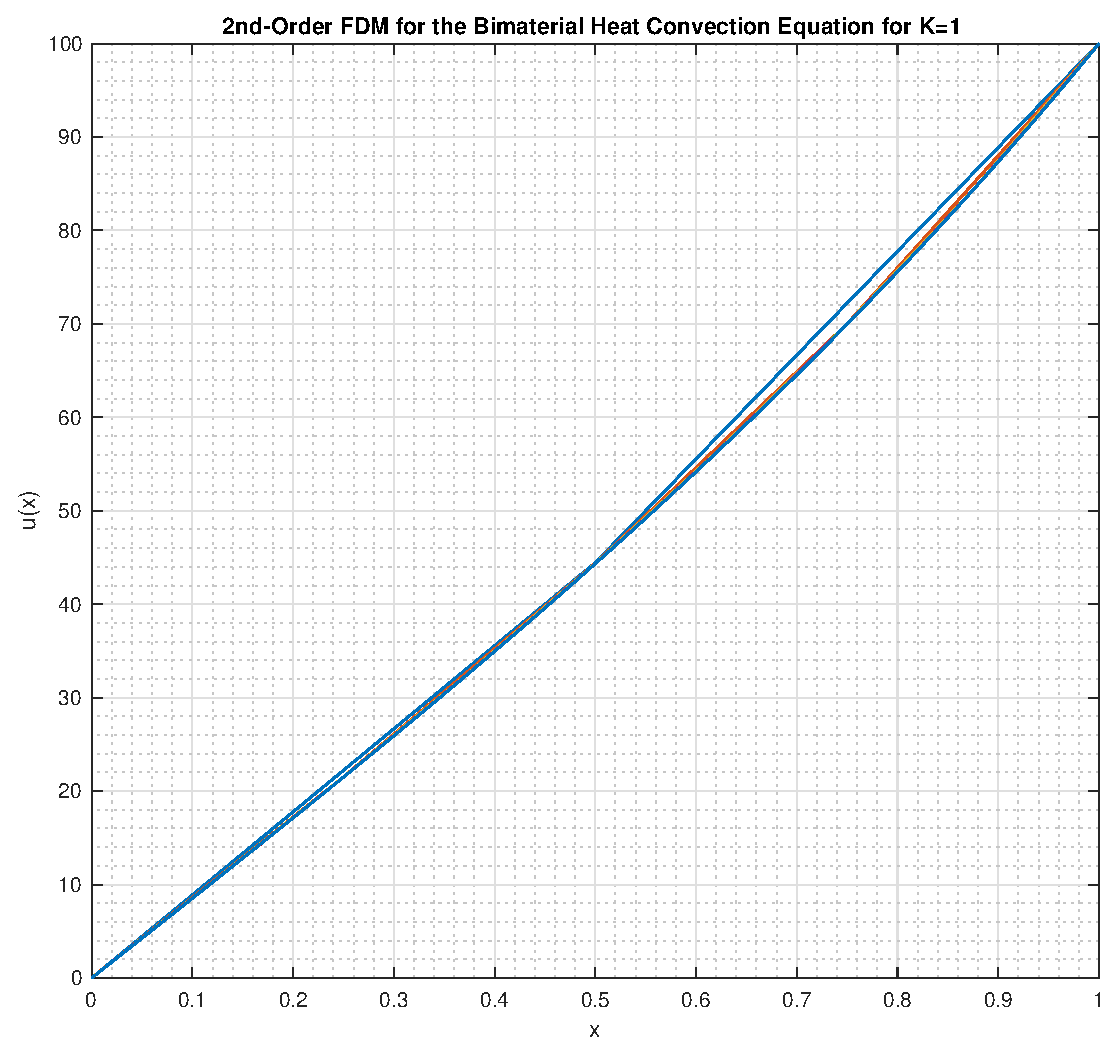
\includegraphics[width=0.6\linewidth]{solution_K_1}
		\caption{FDM Solution for the Bimaterial Heat Convection Equation for K = 1E+0}
	\end{center}
\end{figure}
\vfill
\begin{figure}[H]
	\begin{center}
		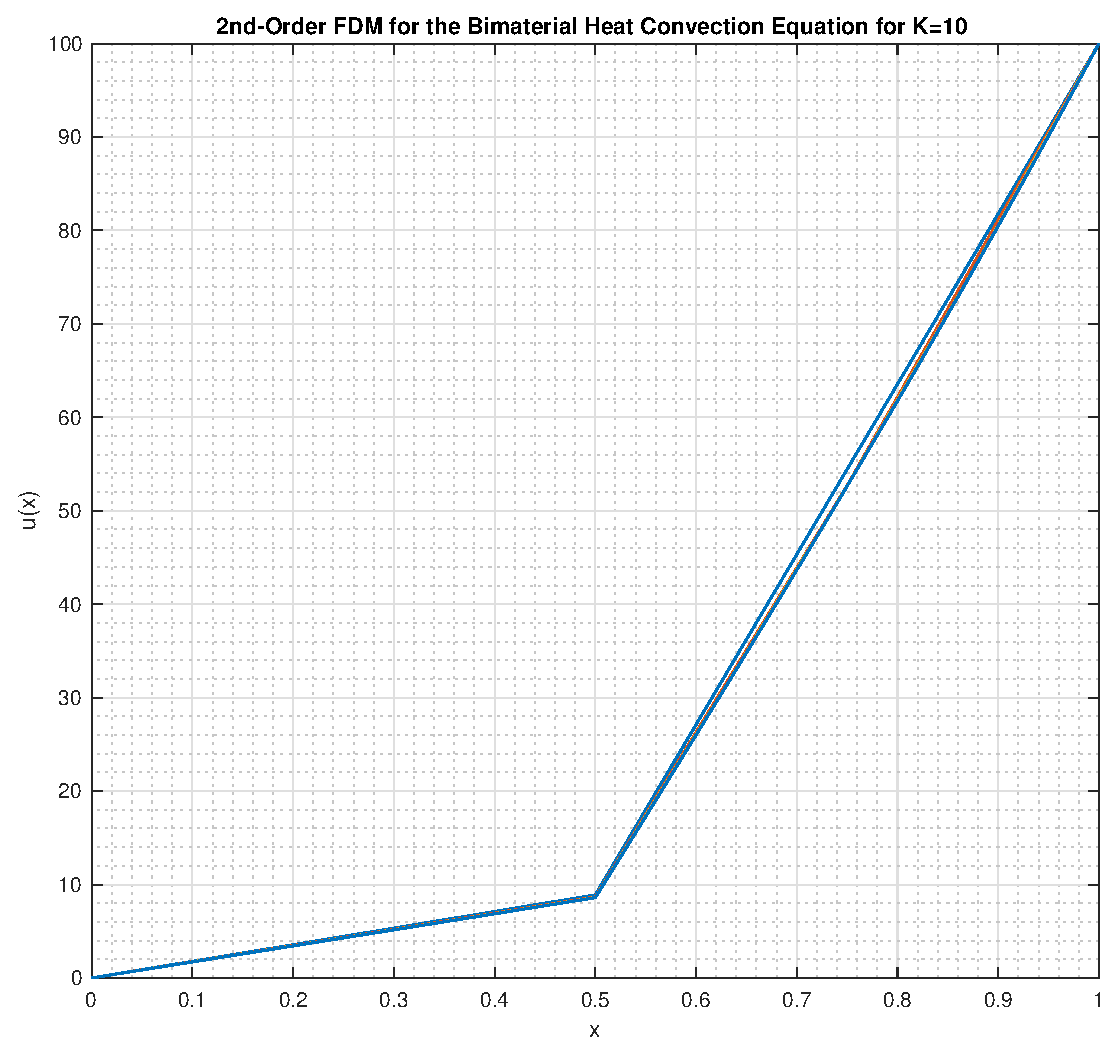
\includegraphics[width=0.6\linewidth]{solution_K_10}
		\caption{FDM Solution for the Bimaterial Heat Convection Equation for K = 1E+1}
	\end{center}
\end{figure}

\begin{figure}[H]
	\begin{center}
		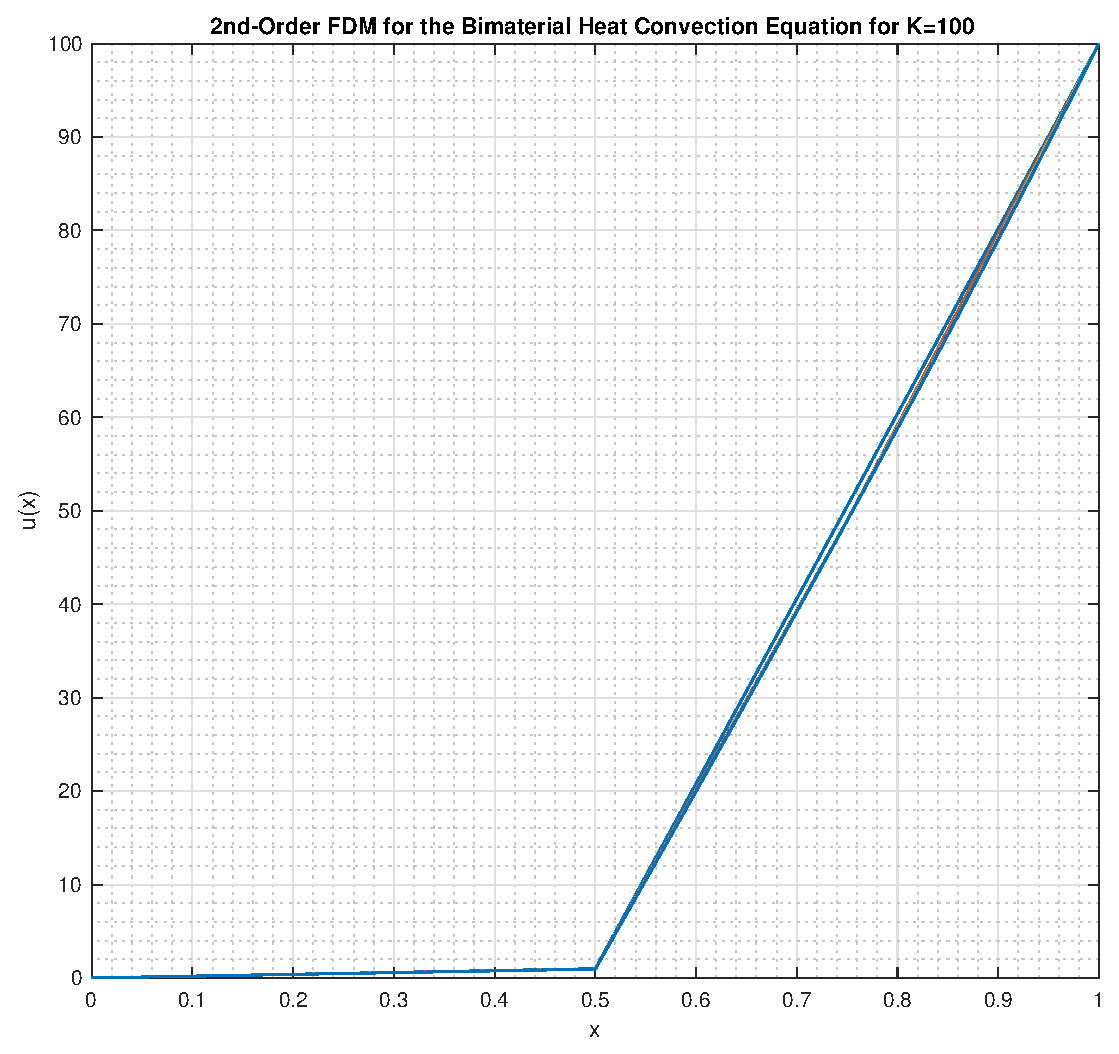
\includegraphics[width=0.6\linewidth]{solution_K_100}
		\caption{FDM Solution for the Bimaterial Heat Convection Equation for K = 1E+2}
	\end{center}
\end{figure}
\vfill
\begin{figure}[H]
	\begin{center}
		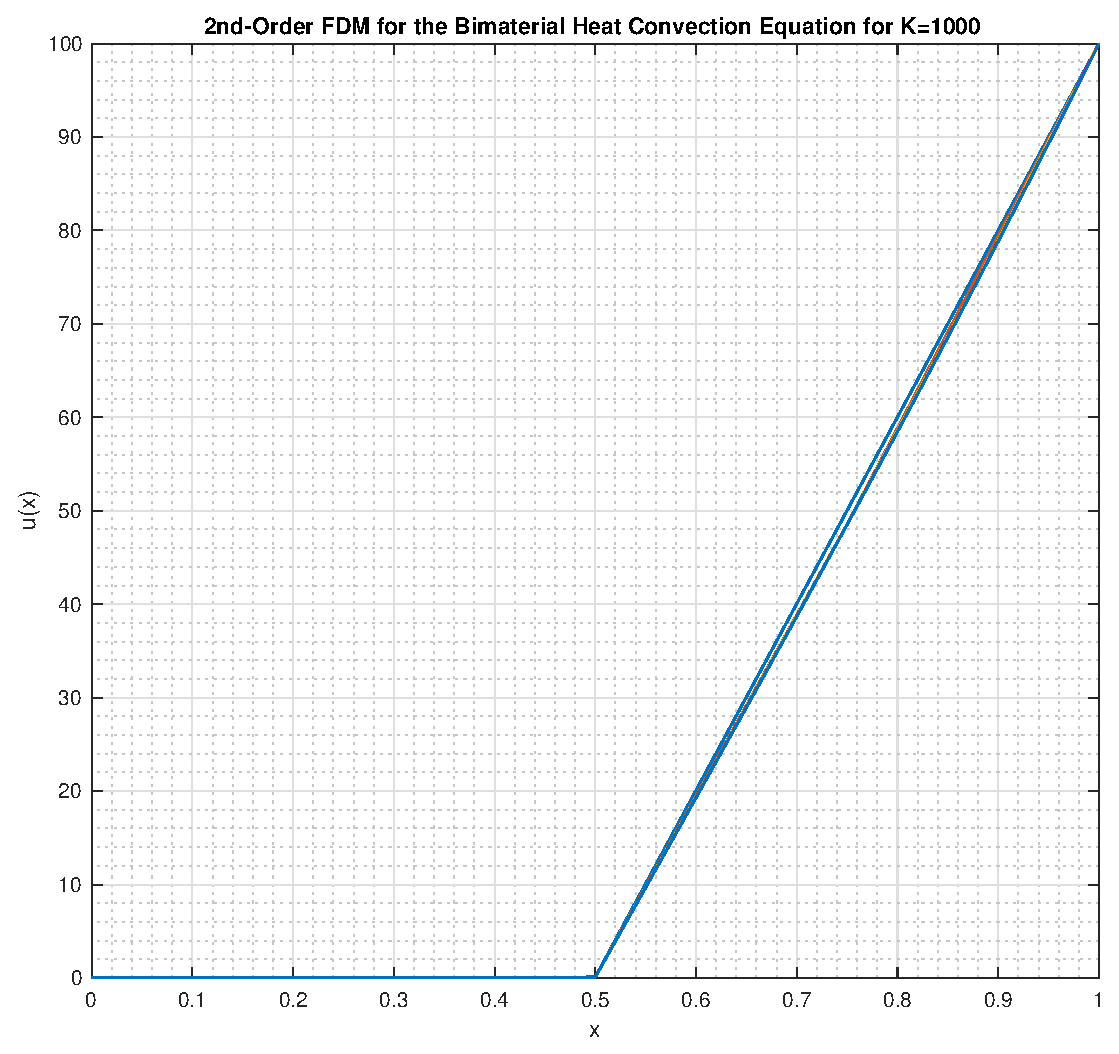
\includegraphics[width=0.6\linewidth]{solution_K_1000}
		\caption{FDM Solution for the Bimaterial Heat Convection Equation for K = 1E+3}
	\end{center}
\end{figure}

\newpage

\subsection*{Rate of Convergence}

Error plots and rate of convergence values are depicted in Figures \ref{fig:conv_temp} and \ref{fig:conv_flux} and tabulated below for the midpoint temperature and the midpoint heat flux. Rate of convergence ($\beta$) values are calculated using a first-order forward difference approximation of the first-derivative of the plot.

\begin{figure}[H]
	\begin{center}
		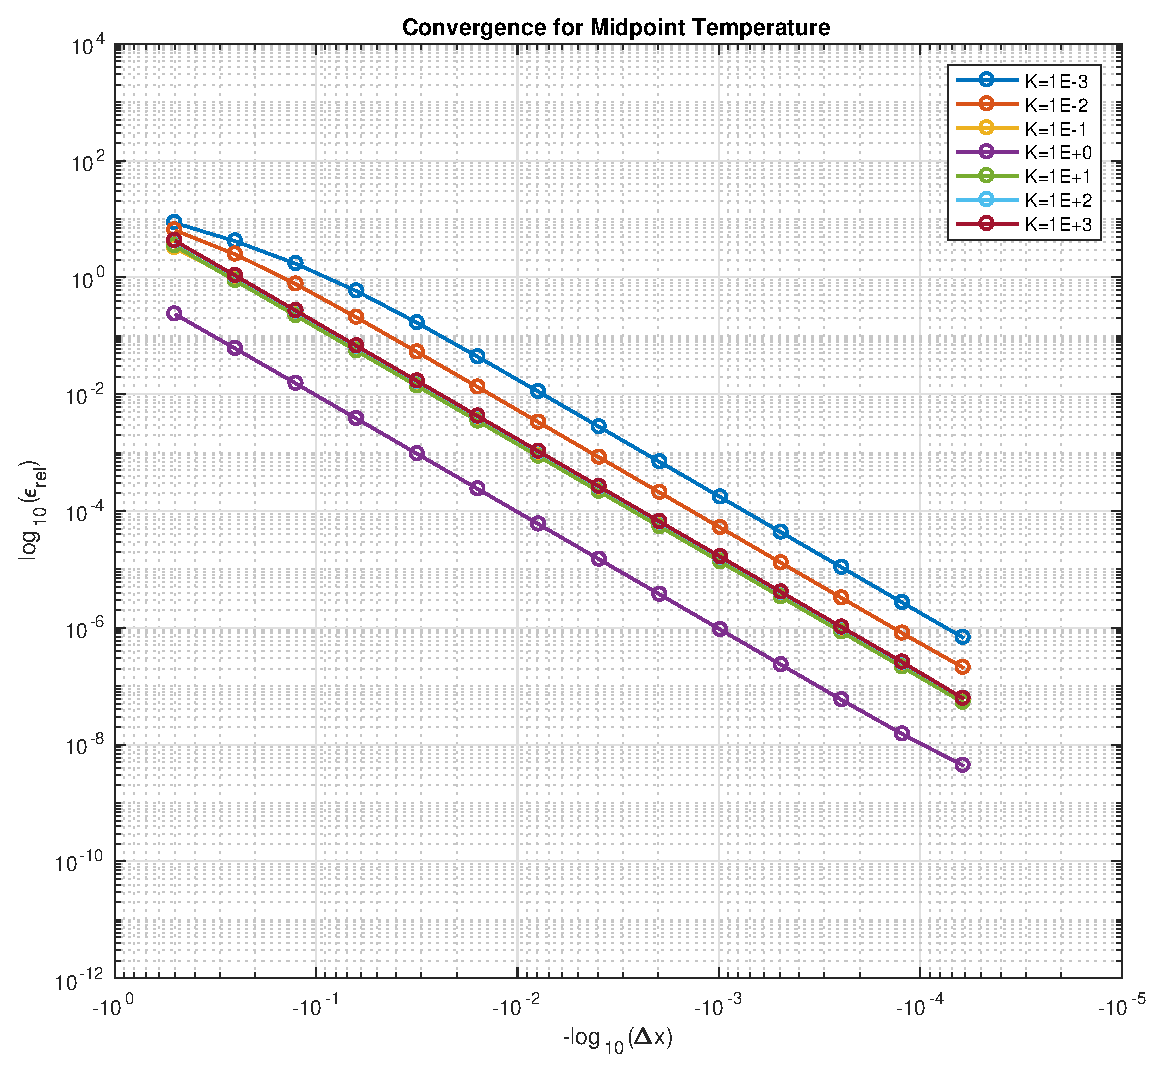
\includegraphics[width=0.6\linewidth]{convergence_u12}
		\caption{FDM Convergence of the Midpoint Temperature}
		\label{fig:conv_temp}
	\end{center}
\end{figure}
\begin{tabular}{|c|c|c|c|c|c|c|c|}
\hline
\textbf{$\Delta x$}&\textbf{$\beta(K=0.001)$}&\textbf{$\beta(K=0.01)$}&\textbf{$\beta(K=0.1)$}&\textbf{$\beta(K=1)$}&\textbf{$\beta(K=10)$}&\textbf{$\beta(K=100)$}&\textbf{$\beta(K=1000)$}\\\hline
0.5000&1.0476&1.3708&1.7958&1.9670&1.9828&1.9906&1.9915\\\hline
0.2500&1.2841&1.6997&1.9408&1.9916&1.9956&1.9976&1.9978\\\hline
0.1250&1.5586&1.8965&1.9845&1.9979&1.9989&1.9994&1.9995\\\hline
0.0625&1.8063&1.9711&1.9961&1.9995&1.9997&1.9998&1.9999\\\hline
0.0312&1.9382&1.9925&1.9990&1.9999&1.9999&2.0000&2.0000\\\hline
0.0156&1.9833&1.9981&1.9998&2.0000&2.0000&2.0000&2.0000\\\hline
0.0078&1.9957&1.9995&1.9999&2.0000&2.0000&2.0000&2.0000\\\hline
0.0039&1.9989&1.9999&2.0000&2.0000&2.0000&2.0000&2.0000\\\hline
0.0020&1.9997&2.0000&2.0000&2.0000&2.0000&2.0000&2.0000\\\hline
0.0010&1.9999&2.0000&2.0001&2.0000&2.0000&2.0000&2.0000\\\hline
0.0005&2.0000&2.0001&1.9998&1.9980&1.9994&2.0003&1.9998\\\hline
0.0002&2.0009&2.0016&1.9954&1.9438&1.9891&2.0001&1.9922\\\hline
0.0001&1.9874&1.9525&1.9618&1.7850&2.0091&2.0208&2.0599\\\hline
0.0001&1.9000&2.0463&0.1843&-2.8450&1.0282&1.8477&2.2216\\\hline
\end{tabular}


\newpage

\begin{figure}[H]
	\begin{center}
		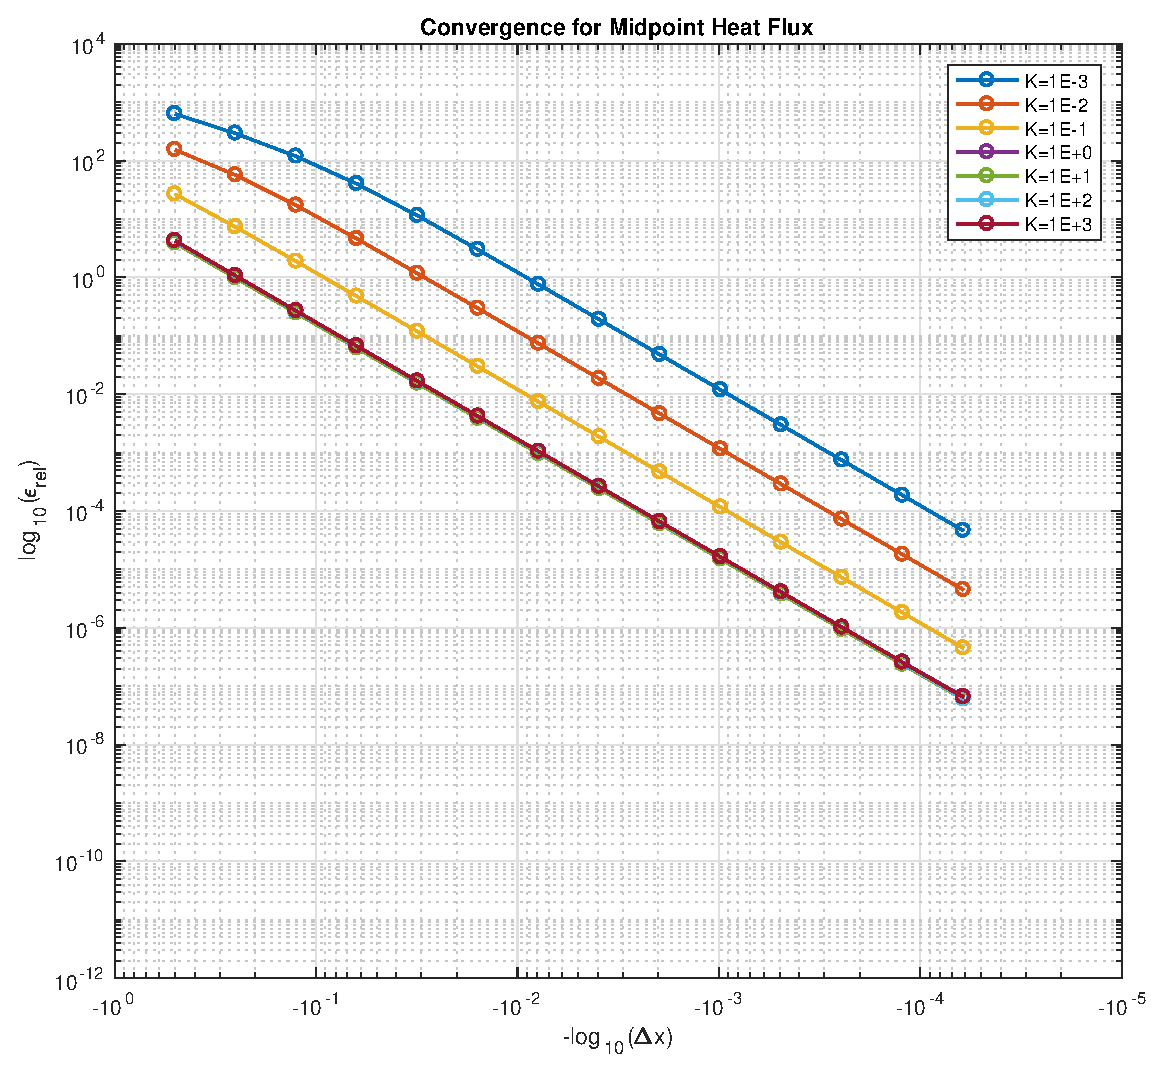
\includegraphics[width=0.6\linewidth]{convergence_Q12}
		\caption{FDM Convergence of the Midpoint Heat Flux}
		\label{fig:conv_flux}
	\end{center}
\end{figure}
\begin{tabular}{|c|c|c|c|c|c|c|c|}
\hline
\textbf{$\Delta x$}&\textbf{$\beta(K=0.001)$}&\textbf{$\beta(K=0.01)$}&\textbf{$\beta(K=0.1)$}&\textbf{$\beta(K=1)$}&\textbf{$\beta(K=10)$}&\textbf{$\beta(K=100)$}&\textbf{$\beta(K=1000)$}\\\hline
0.5000&1.1122&1.4430&1.8705&1.9916&1.9885&1.9912&1.9916\\\hline
0.2500&1.3048&1.7216&1.9608&1.9979&1.9971&1.9977&1.9978\\\hline
0.1250&1.5655&1.9025&1.9896&1.9995&1.9993&1.9994&1.9995\\\hline
0.0625&1.8084&1.9726&1.9974&1.9999&1.9998&1.9999&1.9999\\\hline
0.0312&1.9388&1.9929&1.9993&2.0000&2.0000&2.0000&2.0000\\\hline
0.0156&1.9835&1.9982&1.9998&2.0000&2.0000&2.0000&2.0000\\\hline
0.0078&1.9958&1.9996&2.0000&2.0000&2.0000&2.0000&2.0000\\\hline
0.0039&1.9989&1.9999&2.0000&2.0000&2.0000&2.0000&2.0000\\\hline
0.0020&1.9997&2.0000&2.0000&2.0000&2.0000&2.0000&2.0000\\\hline
0.0010&1.9999&2.0000&2.0000&2.0000&2.0000&2.0000&2.0000\\\hline
0.0005&2.0000&2.0000&2.0000&2.0005&2.0000&2.0000&1.9999\\\hline
0.0002&2.0000&1.9999&2.0005&1.9916&1.9955&2.0017&1.9937\\\hline
0.0001&2.0001&2.0020&2.0061&1.9506&1.9732&2.0636&1.9811\\\hline
0.0001&2.0006&1.9956&2.6006&2.5800&1.9122&1.9256&2.0921\\\hline
\end{tabular}


\newpage

\section*{Conclusion}

Using the second-order central difference scheme and a second-order extraction scheme for the midpoint heat flux, it was shown that the midpoint temperature and the midpoint heat flux demonstrate \textbf{quadratic convergence} ($\beta = 2$). In general, the stiffness variable $K$ of the problem determines the overall conditioning of the interior matrix. That is, for values of $K$ logarithmically far from unity, the value results in poor matrix conditioning which means that it takes a finer mesh to resolve the same amount of error. This is observed in Figure \ref{fig:conv_temp}, where $K=1$ has less relative error for similar mesh sizes compared to all other values of $K$.

\newpage

\appendix

\section*{aero\_430\_hw1\_analytical.m}
\begin{lstlisting}
clear all; close all; clc

set(0,'DefaultFigureWindowStyle','docked')

figure
cmap = colormap(hot);
cIndex = 1;

for K = [1E-3 1E-2 1E-1 1E0 1E1 1E2 1E3]

b = 1;
k2 = 1;
k1 = K*k2;
Ta = 0;
A = 1;

a1 = sqrt(b/k1);
a2 = sqrt(b/k2);

C = [cosh(0) sinh(0) 0 0;
0 0 cosh(a2) sinh(a2);
cosh(a1/2) sinh(a1/2) -cosh(a2/2) -sinh(a2/2);
k1*a1*sinh(a1/2) k1*a1*cosh(a1/2) -k2*a2*sinh(a2/2) -k2*a2*cosh(a2/2)];

d = [-Ta
100-Ta;
0;
0];

aSolCoeff = C\d;


hold on;    box on;
grid on;    grid minor;
x1 = linspace(0.0, 0.5, 100);
x2 = linspace(0.5, 1.0, 100);
s1 = aSolCoeff(1)*cosh(a1*x1) + aSolCoeff(2)*sinh(a1*x1) + Ta;
s2 = aSolCoeff(3)*cosh(a2*x2) + aSolCoeff(4)*sinh(a2*x2) + Ta;
plot([x1 x2], [s1 s2],  'linewidth', 2, 'color', cmap(cIndex, :));
xlim([0 1]);    ylim([0 100]);
title('Analytical Temperature Profile')
xlabel('Distance');  ylabel('Temperature')

cIndex = cIndex + 9;

end

legend('K = 1E-3', 'K = 1E-2', 'K = 1E-1', 'K = 1E+0', 'K = 1E+1', 'K = 1E+2', 'K = 1E+3', ...
'location', 'best') 
saveas(gcf, '430_hw1_analytical_temperature', 'epsc')

figure
cmap = colormap(hot);
cIndex = 1;

for K = [1E-3 1E-2 1E-1 1E0 1E1 1E2 1E3]

b = 1;
k2 = 1;
k1 = K;
Ta = 0;
A = 1;

a1 = sqrt(b/k1);
a2 = sqrt(b/k2);

C = [cosh(0) sinh(0) 0 0;
0 0 cosh(a2) sinh(a2);
cosh(a1/2) sinh(a1/2) -cosh(a2/2) -sinh(a2/2);
k1*a1*sinh(a1/2) k1*a1*cosh(a1/2) -k2*a2*sinh(a2/2) -k2*a2*cosh(a2/2)];

d = [-Ta
100-Ta;
0;
0];

aSolCoeff = C\d;

hold on;    box on;
grid on;    grid minor;
x1 = linspace(0.0, 0.5, 100);
x2 = linspace(0.5, 1.0, 100);
s1 = -k1*A*(aSolCoeff(1)*a1*sinh(a1*x1) + aSolCoeff(2)*a1*cosh(a1*x1));
s2 = -k2*A*(aSolCoeff(3)*a2*sinh(a2*x2) + aSolCoeff(4)*a2*cosh(a2*x2));
plot([x1 x2], [s1 s2],  'linewidth', 2, 'color', cmap(cIndex, :));
xlim([0 1]);    ylim([-inf 0]); 
title('Analytical Heat Flux Profile')
xlabel('Distance');  ylabel('Heat Flux')

cIndex = cIndex + 9;

end

legend('K = 1E-3', 'K = 1E-2', 'K = 1E-1', 'K = 1E+0', 'K = 1E+1', 'K = 1E+2', 'K = 1E+3', ...
'location', 'best') 
saveas(gcf, '430_hw1_analytical_heat_flux', 'epsc')
\end{lstlisting}

\newpage

\section*{aero\_430\_hw1\_fdm.m}
\begin{lstlisting}
% Ross Alexander
% 2.10.18

clc; close all; clear all;

meshOrder   = 1:15;
meshDx      = 0.5.^meshOrder;

rowID = 0;

plotGen         = true;
plotSave        = true;
tableSaveRoc    = true;

%% 2nd-Order FDM

for K = [1E-3 1E-2 1E-1 1E+0 1E+1 1E+2 1E+3]

% Enumerate constants
b = 1;
k2 = 1;
k1 = K*k2;

rowID = rowID + 1;
colID = 0;

if plotGen

xlabel('x');    ylabel('u(x)');
grid on;        grid minor;
box on;         hold on;
set(gcf, 'Position', [1 1 624 550])

titleString = strcat('2nd-Order FDM for the Bimaterial Heat Convection Equation for K=', ...
num2str(K));
title(titleString)

end

for dx = meshDx

% Develop mesh-specific values for FDM calculations
nxi = 1 / dx - 1;               % number of interior nodes
nxt = 1 / dx + 1;               % number of total nodes (includes boundary nodes)
xi = linspace(dx, 1-dx, nxi);   % x-values at interior nodes
xt = linspace(0, 1, nxt);       % x-values at total nodes
f = zeros(nxi, 1);              % interior load vector
colID = colID + 1;

nxiHalf = (nxi+1)/2;            % index for central interior node (x = 1/2) rel. to interior
nxtHalf = (nxt+1)/2;            % index for central interior node (x = 1/2) rel. to total

% Enumerate upper matrix and lower matrix constants
alpha1 = -k1;                       alpha2 = -k2;           % subdiagonal values
beta1  = b*dx^2+2*k1;               beta2  = b*dx^2+2*k2;   % diagonal values
gamma1 = -k1;                       gamma2 = -k2;           % superdiagonal values

if dx ~= 1/2

% Construct upper matrix and lower matrix
A1 = gallery('tridiag', nxiHalf, alpha1, beta1, gamma1);    % upper matrix for k1
A2 = gallery('tridiag', nxiHalf, alpha2, beta2, gamma2);    % lower matrix for k2

% Construct central vector for node at x = 1/2 for k1 and k2
a = zeros(1, nxi);
a(nxiHalf - 1) = -k1;
a(nxiHalf)     = b*dx^2+k1+k2;
a(nxiHalf + 1) = -k2;

% Assemble entire interior matrix by combining upper, central, and lower matrices
A = [A1(1:end-1, :) zeros(nxiHalf-1, nxiHalf-1);
a; 
zeros(nxiHalf-1, nxiHalf-1) A2(2:end, :)];

% Enumerate load values at boundary nodes
f(1) = 0;       f(nxi) = 100*k2;

else

% If dx = 1/2 the solution is trivial
A = b*dx^2+k1+k2;
f = k2*100;

end

% Solve for u and append values at boundary nodes
ui = A\f;
ut = [0; ui; 100];

if plotGen && dx >= meshDx(8)
plot(xt, ut, 'linewidth', 1)
end

%% Quantities of Interest

% Develop analytical solution and corresponding coefficients
a1 = sqrt(b/k1);
a2 = sqrt(b/k2);

C = [cosh(0) sinh(0) 0 0;
0 0 cosh(a2) sinh(a2);
cosh(a1/2) sinh(a1/2) -cosh(a2/2) -sinh(a2/2);
k1*a1*sinh(a1/2) k1*a1*cosh(a1/2) -k2*a2*sinh(a2/2) -k2*a2*cosh(a2/2)];

d = [0
100;
0;
0];

aSolCoeff = C\d;

% Calculate midpoint temperature and heat flux from analytical and FDM solutions
u12.exact(rowID, colID) = aSolCoeff(1)*cosh(a1/2) + aSolCoeff(2)*sinh(a1/2);
u12.fdm(rowID, colID)   = ut(nxtHalf);
Q12.exact(rowID, colID) = -k1*(aSolCoeff(1)*a1*sinh(a1/2) + aSolCoeff(2)*a1*cosh(a1/2));
Q12.fdm(rowID, colID)   = -k1*(ut(nxtHalf)-ut(nxtHalf-1))/dx - b*dx/2*ut(nxtHalf);           % Q-
%         Q12.fdm(rowID, colID)   = -k2*(ut(nxtHalf+1)-ut(nxtHalf))/dx + b*dx/2*ut(nxtHalf); % Q+

end

if plotGen

%         legend('\Deltax = (1/2)^1', '\Deltax = (1/2)^2', '\Deltax = (1/2)^3', ...
%             '\Deltax = (1/2)^4', '\Deltax = (1/2)^5', '\Deltax = (1/2)^6', ...
%             '\Deltax = (1/2)^7', '\Deltax = (1/2)^8', ...
%             'location', 'eastoutside')

drawnow

if plotSave

figureString = strcat('solution_K_', num2str(rowID));
saveas(gcf, figureString, 'epsc')

close gcf

end

end

end

%% Convergence Plotting

% Calculate relative error
relErroru12 = abs(u12.exact-u12.fdm) ./ abs(u12.exact) * 100;
relErrorQ12 = abs(Q12.exact-Q12.fdm) ./ abs(Q12.exact) * 100;

if plotGen

%%% Midpoint Temperature

fig2 = figure(2);
xlabel('-log_{10}(\Deltax)');   ylabel('log_{10}(\epsilon_{rel})');
grid on;                        grid minor;
box on;                         hold on;
ylim([10^-12 10^4])
set(gcf, 'Position', [1 1 624 550])

% Plot log-log relative error in midpoint temperature v. -mesh size
for KID = 1:7
loglog(-meshDx, relErroru12(KID, :), '-o', 'linewidth', 1.25);
end

titleString = strcat('Convergence for Midpoint Temperature');
title(titleString)

legend('K=1E-3', 'K=1E-2', 'K=1E-1', 'K=1E+0', 'K=1E+1', 'K=1E+2', 'K=1E+3')

set(gca, 'XScale', 'log');  set(gca, 'YScale', 'log');
drawnow

%%% Midpoint Heat Flux

fig3 = figure(3);
xlabel('-log_{10}(\Deltax)');   ylabel('log_{10}(\epsilon_{rel})');
grid on;                        grid minor;
box on;                         hold on;
ylim([10^-12 10^4])
set(gcf, 'Position', [1 1 624 550])

% Plot log-log relative error in midpoint heat flux v. -mesh size
for KID = 1:7
loglog(-meshDx, relErrorQ12(KID, :), '-o', 'linewidth', 1.25);
end

titleString = strcat('Convergence for Midpoint Heat Flux');
title(titleString)

legend('K=1E-3', 'K=1E-2', 'K=1E-1', 'K=1E+0', 'K=1E+1', 'K=1E+2', 'K=1E+3')

set(gca, 'XScale', 'log');  set(gca, 'YScale', 'log');
drawnow

if plotSave

figure(2)
saveas(gcf, 'convergence_u12', 'epsc')

figure(3)
saveas(gcf, 'convergence_Q12', 'epsc')

end

end

%% Rate of Convergence Determination

logRelErroru12 = log10(relErroru12);

for KID = 1:7

for rocID = 1:length(logRelErroru12) - 1
rocu12(KID, rocID) = (logRelErroru12(KID, rocID+1) - logRelErroru12(KID, rocID)) / -log10(2);
end

end

if tableSaveRoc

colLabelsRoc = {'$\Delta x$', '$\beta(K=0.001)$', '$\beta(K=0.01)$', '$\beta(K=0.1)$', ...
'$\beta(K=1)$', '$\beta(K=10)$', '$\beta(K=100)$', '$\beta(K=1000)$'};
matrix2latex([meshDx(1:length(meshOrder)-1)' rocu12'], 'roc_u12.tex', ...
'columnLabels', colLabelsRoc, 'alignment', 'c', 'format', '%5.4f')

end

logRelErrorQ12 = log10(relErrorQ12);

for KID = 1:7

for rocID = 1:length(logRelErrorQ12) - 1
rocQ12(KID, rocID) = (logRelErrorQ12(KID, rocID+1) - logRelErrorQ12(KID, rocID)) / -log10(2);
end

end

if tableSaveRoc

colLabelsRoc = {'$\Delta x$', '$\beta(K=0.001)$', '$\beta(K=0.01)$', '$\beta(K=0.1)$', ...
'$\beta(K=1)$', '$\beta(K=10)$', '$\beta(K=100)$', '$\beta(K=1000)$'};
matrix2latex([meshDx(1:length(meshOrder)-1)' rocQ12'], 'roc_Q12.tex', ...
'columnLabels', colLabelsRoc, 'alignment', 'c', 'format', '%5.4f')

end
\end{lstlisting}

\section*{matrix2latex.m}
\begin{lstlisting}
function matrix2latex(matrix, filename, varargin)

% function: matrix2latex(...)
% Author:   M. Koehler
% Contact:  koehler@in.tum.de
% Version:  1.1
% Date:     May 09, 2004

% This software is published under the GNU GPL, by the free software
% foundation. For further reading see: http://www.gnu.org/licenses/licenses.html#GPL

% Usage:
% matrix2late(matrix, filename, varargs)
% where
%   - matrix is a 2 dimensional numerical or cell array
%   - filename is a valid filename, in which the resulting latex code will
%   be stored
%   - varargs is one ore more of the following (denominator, value) combinations
%      + 'rowLabels', array -> Can be used to label the rows of the
%      resulting latex table
%      + 'columnLabels', array -> Can be used to label the columns of the
%      resulting latex table
%      + 'alignment', 'value' -> Can be used to specify the alginment of
%      the table within the latex document. Valid arguments are: 'l', 'c',
%      and 'r' for left, center, and right, respectively
%      + 'format', 'value' -> Can be used to format the input data. 'value'
%      has to be a valid format string, similar to the ones used in
%      fprintf('format', value);
%      + 'size', 'value' -> One of latex' recognized font-sizes, e.g. tiny,
%      HUGE, Large, large, LARGE, etc.
%
% Example input:
%   matrix = [1.5 1.764; 3.523 0.2];
%   rowLabels = {'row 1', 'row 2'};
%   columnLabels = {'col 1', 'col 2'};
%   matrix2latex(matrix, 'out.tex', 'rowLabels', rowLabels, 'columnLabels', ...
%       columnLabels, 'alignment', 'c', 'format', '%-6.2f', 'size', 'tiny');
%
% The resulting latex file can be included into any latex document by:
% /input{out.tex}
%
% Enjoy life!!!

rowLabels = [];
colLabels = [];
alignment = 'l';
format = [];
textsize = [];
if (rem(nargin,2) == 1 || nargin < 2)
error('matrix2latex: ', 'Incorrect number of arguments to %s.', mfilename);
end

okargs = {'rowlabels','columnlabels', 'alignment', 'format', 'size'};
for j=1:2:(nargin-2)
pname = varargin{j};
pval = varargin{j+1};
k = strmatch(lower(pname), okargs);
if isempty(k)
error('matrix2latex: ', 'Unknown parameter name: %s.', pname);
elseif length(k)>1
error('matrix2latex: ', 'Ambiguous parameter name: %s.', pname);
else
switch(k)
case 1  % rowlabels
rowLabels = pval;
if isnumeric(rowLabels)
rowLabels = cellstr(num2str(rowLabels(:)));
end
case 2  % column labels
colLabels = pval;
if isnumeric(colLabels)
colLabels = cellstr(num2str(colLabels(:)));
end
case 3  % alignment
alignment = lower(pval);
if alignment == 'right'
alignment = 'r';
end
if alignment == 'left'
alignment = 'l';
end
if alignment == 'center'
alignment = 'c';
end
if alignment ~= 'l' && alignment ~= 'c' && alignment ~= 'r'
alignment = 'l';
warning('matrix2latex: ', 'Unkown alignment. (Set it to \''left\''.)');
end
case 4  % format
format = lower(pval);
case 5  % format
textsize = pval;
end
end
end

fid = fopen(filename, 'w');

width = size(matrix, 2);
height = size(matrix, 1);

if isnumeric(matrix)
matrix = num2cell(matrix);
for h=1:height
for w=1:width
if(~isempty(format))
matrix{h, w} = num2str(matrix{h, w}, format);
else
matrix{h, w} = num2str(matrix{h, w});
end
end
end
end

if(~isempty(textsize))
fprintf(fid, '\\begin{%s}', textsize);
end

fprintf(fid, '\\begin{tabular}{|');

if(~isempty(rowLabels))
fprintf(fid, 'l|');
end
for i=1:width
fprintf(fid, '%c|', alignment);
end
fprintf(fid, '}\r\n');

fprintf(fid, '\\hline\r\n');

if(~isempty(colLabels))
if(~isempty(rowLabels))
fprintf(fid, '&');
end
for w=1:width-1
fprintf(fid, '\\textbf{%s}&', colLabels{w});
end
fprintf(fid, '\\textbf{%s}\\\\\\hline\r\n', colLabels{width});
end

for h=1:height
if(~isempty(rowLabels))
fprintf(fid, '\\textbf{%s}&', rowLabels{h});
end
for w=1:width-1
fprintf(fid, '%s&', matrix{h, w});
end
fprintf(fid, '%s\\\\\\hline\r\n', matrix{h, width});
end

fprintf(fid, '\\end{tabular}\r\n');

if(~isempty(textsize))
fprintf(fid, '\\end{%s}', textsize);
end

fclose(fid);
\end{lstlisting}

\end{document}